%%%%%%%%%%%%%%%%%%%%%%%%%%%%%%%%%%%%%%%%%%%%%%%%%%%%%%%%%%%%%%%%%%%%%
% University Assignment Title Page 
% LaTeX Template
% Version 1.0 (27/12/12)
%
% This template has been downloaded from:
% http://www.LaTeXTemplates.com
%
% Original author:
% WikiBooks (http://en.wikibooks.org/wiki/LaTeX/Title_Creation)
%
% License:
% CC BY-NC-SA 3.0 (http://creativecommons.org/licenses/by-nc-sa/3.0/)
%%%%%%%%%%%%%%%%%%%%%%%%%%%%%%%%%%%%%%%%%%%%%%%%%%%%%%%%%%%%%%%%%%%%%

\documentclass[11pt,canadien]{article}

\usepackage{babel} % Pour la typo canadienne
\usepackage{graphviz} % Pour inclure des images
\usepackage[utf8]{inputenc} % Pour les accents sur le document
\usepackage{mathptmx} % Pour Times New Roman
\usepackage[top=1in,bottom=1in,left=1in,right=1in]{geometry} % Marges de 1 pouce
\usepackage[toc,page]{appendix} % Pour avoir des annexes et qui figures sur le sommaire
\usepackage{float} % Pour placer précisement les figures (notament la position 'H')
\usepackage{titlesec} % Pour sauter les pages à chaque section

\begin{document}

\newcommand{\sectionbreak}{\clearpage} % Applique le saut de page à chaque section
\newcommand{\code}[1]{\vspace{0.2cm} \texttt{#1}} % Créer une commande pour insérer du code

% Membres du groupe
\newcommand{\antoine}{Antoine \textsc{Moreau}}
\newcommand{\estelle}{Estelle \textsc{Michel}}
\newcommand{\joffrey}{Joffrey \textsc{Germain}}
\newcommand{\julien}{Julien \textsc{Naty-Daufin}}
\newcommand{\karen}{Karen \textsc{Migan}}
\newcommand{\kevin}{Kévin \textsc{Seroux}}
\newcommand{\valentin}{Valentin \textsc{Tertois}}

\begin{titlepage}

\newcommand{\HRule}{\rule{\linewidth}{0.5mm}} % Defines a new command for the horizontal lines, change thickness here

\center % Center everything on the page
 
%-----------------
% HEADING SECTIONS
%-----------------


\includegraphics[width=\textwidth]{images/uqac_logo.jpg} % logo
 
\textsc{\LARGE 8IFG145 - Gestion de projets informatique}\\[0.5cm]

%--------------
% TITLE SECTION
%--------------

\HRule \\[0.4cm]
{ \huge \bfseries TP1 - Compréhension et exécution de commandes avec GitHub}\\[0.4cm]
\HRule \\[0.5cm]
 
%---------------
% AUTHOR SECTION
%---------------

\begin{minipage}{0.4\textwidth}
\begin{flushleft} \large
\emph{Étudiants :}
\\ \antoine
\\ \estelle
\\ \joffrey
\\ \julien
\\ \karen
\\ \kevin
\\ \valentin
\end{flushleft}
\end{minipage}
~
\begin{minipage}{0.4\textwidth}
\begin{flushright} \large
\emph{Professeur :}\\
Dany \textsc{Fortin-Simard}
\end{flushright}
\end{minipage}\\[2cm]

%-------------
% DATE SECTION
%-------------

{\large \today}\\[2cm]

\vfill % Fill the rest of the page with whitespace

\end{titlepage}

\newpage
\tableofcontents

\section{Introduction au langage Git et à l'outil Github}
Blablabla

\section{Apprentissage de Github}
Les commandes \texttt{merge}, \texttt{fetch}, \texttt{pull}, \texttt{push} prennent facultativement en argument le dépôt distant (ex: origin) et la branche distante (ex: master).

\paragraph{git commit}Cette commande est une des commandes principales de l'outil git, elle permet de stocker le contenu de l'index et de "valider" les changements apportés aux fichiers présents dans le dépot. Habituellement, lors de l'exécution de la commande, l'utilisateur utilise l'option \texttt{-m 'Mon texte'} afin de décrire les modifications apportés par cette nouvelle version des fichiers.
\begin{figure}[H]
	\centering
	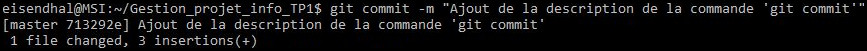
\includegraphics[width=\textwidth]{images/git_commit.jpg}
\end{figure}

\paragraph{git merge}Cette commande permet de fusionner deux branches. Cette commande va fusionner les commits des deux branches depuis leur séparation, le résultat de cette commande est qu'il ne restera plus qu'une branche, intégrant les modifications apportées par les deux branches. L'option \texttt{-m 'Mon texte'} permet de préciser le message du commit qui sera effectué lors de la fusion des deux branches.
\begin{figure}[H]
	\centering
	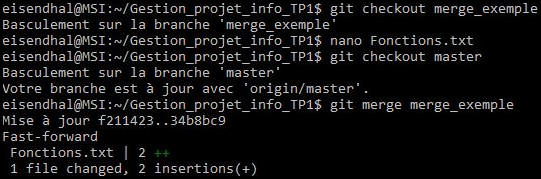
\includegraphics[width=\textwidth]{images/git_merge.jpg}
\end{figure}

\paragraph{git cherry-pick}Cette commande permet d'appliquer les modifications d'un commit particulier d'une autre branche à la branche actuelle. Par exemple, si un correctif a été développé sur une autre branche, et qu'il devient nécessaire
de le déployer sur la branche principale, il est possible, grâce à \texttt{cherry-pick}, de ne récupérer que les modifications apportées par le commit qui nous intéresse.
\begin{figure}[H]
	\centering
	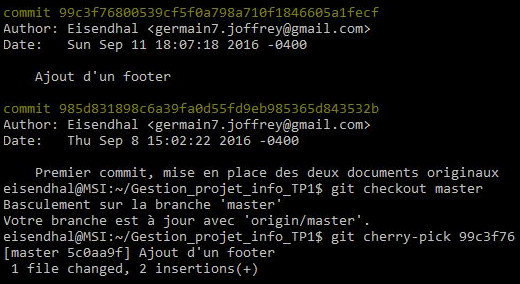
\includegraphics[width=\textwidth]{images/git_cherry-pick.jpg}
\end{figure}

\paragraph{git status}La commande permet d'afficher les chemins qui ont des differences entre le fichier index et le HEAD commit actuelle mais aussi les chemins qui ont des différences entre l'arbre actuelle et le fichier d'index et enfin les chemins l'abre actuel qui ne sont pas retenu par GIT. Les premiers chemins correspondent à ce que vous utiliseriez en faisent un git-commit tous les autre correspondent quand à eux à un git-add suivi d'un git-commit. L'option \texttt{-s} ou \texttt{--short} permet de formater l'affichage de la commande dans le format \texttt{short}.

\paragraph{git log}Permet d'afficher les logs (le journal) des commits. La commande utilise les options applicable à la commande \texttt{git rev-list} afin de controler ce qui est afficher et comment, ainsi que les options applicable à la commande \texttt{git diff -*} afin de controler l'affichage des changement induit par  chaque commit.

\paragraph{git tag}La commande permet de créer, lister, supprimer ou de verifier un objet "tag" encoder avec la clé GPG. Par exemple si l'on veut supprimer on utilisera  l'option \texttt{-d}, si l'on veut lister on utilisera l'option \texttt{-l} et si l'on veut verifier on utilisera l'option \texttt{-v}.

\paragraph{git branch}La commande permet de gérer tout ce qui a attrait aux branches (ajout, listing, suppression, renommage). On ne peut cependant  pas supprimer une branche qui n'aurait pas été fusionné avec une autre (on perdrait alors les modifications de la branche). Si on souhaite forcer cette suppression, et perdre tout le travail effectué dessus il faudra utiliser un D majuscule.
\code{
\\	git branch               \# Permet de lister les branches
\\	git branch <branche>     \# Permet de créer une nouvelle branche <branche>
\\	git branch -m <branche>  \# Renomme la branche courante en <branche>
\\	git branch -d <branche>  \# Permet de supprimer une branche
\\	git branch -D <branche>  \# Supprime la branche même si elle n'a pas été fusionnée
}

\paragraph{git checkout}Une fois les branches créées, il faut être capable d'aller d'une branche à une autre. Pour cela, on peut compter sur la commande ``checkout''. \texttt{git checkout <branche>} permet de se rendre sur une branche existante. En revanche, si vous le souhaitez, vous pouvez demander à git de sauter sur une branche qui n'existe pas en la créant au préalable.
\code{
\\	git checkout -b <branche> \# est équivalent à :
\\	git branch <branche>
\\	git checkout <branche>
}

\paragraph{git diff}Comme son nom l’indique, elle permet de voir les changements entre deux versions de fichiers (l’ancienne modifiée et l’actuelle) lors de la correction d’un bug ou l’ajout d’une fonctionnalité par exemples. Les lignes ajoutées sont donc précédées d’un « + » tandis que les lignes supprimées sont précédées d’un « - ». Normalement les lignes sont colorées et donc faciles à repérer. Par défaut, Git affiche les modifications de tous les fichiers qui ont changé. Vous pouvez demander à Git d’afficher seulement les changements d’un fichier précis, comme ceci :
git diff chemin vers le fichier

\paragraph{git fetch}Mise à jour des références locales des branches distantes ainsi que des objets git (commit principalement). Dit autrement, elle permet au dépôt local, de prendre simplement conscience des modifications distantes. Elles ne sont pas appliquées aux branches locales. Cette commande est sûre.
\begin{figure}[H]
	\centering
	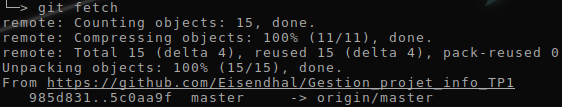
\includegraphics{images/git_fetch.png}
\end{figure}

\paragraph{git pull}Exécution d'un \texttt{git fetch} puis d'un \texttt{git merge}. Bien qu'elle soit pratique, quand la branche locale n'est pas derrière la branche distante, des fusions (avec commits parfois) sont effectués sans pouvoir annuler. Ce qui pose un soucis, pour la lisibilité de l'historique d'un dépôt. Il est d'usage d'utiliser plutôt \texttt{git pull --rebase} afin de remplacer l'opération de merging en une opération de rebasing. Il existe plusieurs façons par \texttt{git config} de spécifier ce comportement par défaut.
\begin{figure}[H]
	\centering
	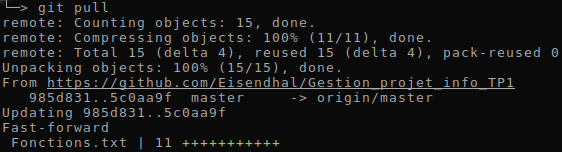
\includegraphics{images/git_pull.png}
\end{figure}

\paragraph{git push}Mise à jour des références du dépôt distant ainsi que des objets git (commit principalement). Dit autrement, elle permet au dépôt distant, d'appliquer les modifications locales. Il pourrait s'agir d'un git pull côté distant, sauf que c'est un autre dépôt qui est à l'initiative. Même si c'est rarement une bonne idée, on peut forcer le push si les branches locales et distantes ne sont pas cohérentes avec l'option \texttt{-f}.
\begin{figure}[H]
	\centering
	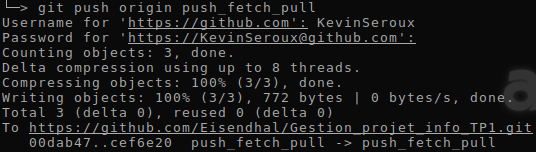
\includegraphics{images/git_push.png}
\end{figure}

\section{Utilisation de Github}
Blablabla

\newpage
\begin{appendices} % Les annexes commencent

\section{Répartition des différentes tâches}
\begin{tabular}{l l l l}
	\textbf{Tâche} & \textbf{Temps} & \textbf{Date d'échéance} & \textbf{Responsable}
	\\ \hline
	   Partie 2 - Présentation de Git       & 3h    & 2016-09-22 & \antoine
	\\ Mise en forme du document final      & 3h    & 2016-10-04 & \kevin
	\\ Mise en place du dépôt Git et droits & 45min & 2016-09-08 & \joffrey
	\\ Description \texttt{git add}         & 30min & 2016-09-15 & \estelle
	\\ Description \texttt{git mv}          & 30min & 2016-09-15 & \estelle
	\\ Description \texttt{git rm}          & 30min & 2016-09-15 & \estelle
	\\ Description \texttt{git init}        & 30min & 2016-09-15 & \julien
	\\ Description \texttt{git clone}       & 30min & 2016-09-15 & \julien
	\\ Description \texttt{git rebase}      & 30min & 2016-09-15 & \julien
	\\ Description \texttt{git status}      & 30min & 2016-09-15 & \valentin
	\\ Description \texttt{git log}         & 30min & 2016-09-15 & \valentin
	\\ Description \texttt{git tag}         & 30min & 2016-09-15 & \valentin
	\\ Description \texttt{git commit}      & 30min & 2016-09-15 & \joffrey
	\\ Description \texttt{git merge}       & 30min & 2016-09-15 & \joffrey
	\\ Description \texttt{git cherry-pick} & 30min & 2016-09-15 & \joffrey
	\\ Description \texttt{git diff}        & 30min & 2016-09-15 & \karen
	\\ Description \texttt{git branch}      & 30min & 2016-09-15 & \karen
	\\ Description \texttt{git checkout}    & 30min & 2016-09-15 & \karen
	\\ Description \texttt{git push}        & 30min & 2016-09-15 & \kevin
	\\ Description \texttt{git fetch}       & 30min & 2016-09-15 & \kevin
	\\ Description \texttt{git pull}        & 30min & 2016-09-15 & \kevin
	\\ Description \texttt{git stash}       & 30min & 2016-09-15 & \antoine
	\\ Description \texttt{git reset}       & 30min & 2016-09-15 & \antoine
	\\ \ldots
	\\ Correction orthographique du rapport & 1h    & 2016-10-04 & Grammar Nazi (Joffrey)
	\\ Évaluation du groupe                 & 45min & \ldots     & Tous
	\\ Présentation orale                   & 5min  & 2016-10-04 & Estelle, Julien, Valentin
\end{tabular}

\section{Évaluation des membres}
Blablabla

\end{appendices}

\end{document}
